% !TeX encoding = UTF-8
% !TeX spellcheck = en_US

\chapter{Evaluation}
\label{evaluation}
This chapter evaluates the implementation of eMoflon::IBeX-GT with respect to the following criteria:
\begin{itemize}
	\item compliance with the requirements from Chapter~\ref{requirements}, \ie whether all requirements for the tool are met or not (see Section~\ref{evaluation-requirements}),
	\item correctness of the graph transformation API, \ie whether the correct matches are found and the rules are applied as defined by the semantics or not (see Section~\ref{evaluation-correctness}),
	\item correctness of the validation of the rule specification in the textual editor, \ie whether the user gets feedback for faulty specifications or not (see Section~\ref{evaluation-validation}),
	\item performance/scalability depending on model size (see Section~\ref{evaluation-performance}),
	\item and feedback on the usability of the eMoflon::IBeX-GT received from actual end-users (see Section~\ref{evaluation-usability}).
\end{itemize}


\section{Compliance with the Requirements}
\label{evaluation-requirements}
In Chapter~\ref{requirements} we presented a list of requirements which are checked for eMoflon::IBeX-GT in the following.

\begin{description}
	\item[Incrementality] ~\\
		eMoflon::IBeX-GT uses an incremental pattern matching engine.
		Section~\ref{incrementality} presents how the incrementality of the engine can be used to support incremental features in the API.

	\item[Interpreter] ~\\
		The eMoflon::IBeX-GT interpreter is used by the API to realize model queries and transformations.
		It can be used without the API if someone prefers to deal with type casting in his/her code directly.

	\item[Integration with a TGG tool] ~\\
		eMoflon::IBeX-GT is integrated into the eMoflon::IBeX tool suite which combines a GT and a TGG tool with some shared libraries.
		After refactoring the TGG part to use the IBeX pattern model as well (cp. Section~\ref{shared-patterns}) even larger parts of the code can be shared.

	\item[Mature integration with a general purpose language] ~\\
		The API is a typed interface for the graph transformation interpreter.
		This allows to a type-safe invocation of model queries and rule applications.

	\item[Dedicated support for model queries] ~\\
		Matches for patterns and rules can be queried via the API.

	\item[DPO or SPO semantics] ~\\
		The API uses with SPO semantics by default, which can be changed to DPO (see Section~\ref{api-pushout-approaches}).
		The pushout approach can be set for the whole API, a rule or just a single rule application.

	\item[Modularity on rule level] ~\\
		Pattern refinement (see Section~\ref{pattern-refinement}) has been implemented to support modularity on rule level.

	\item[Application conditions] ~\\
		The new graph transformation tool has mature support for positive and negative application conditions, which can be combined via OR and AND (with the only restriction that one must define the logical expressions in DNF).
	
	\item[Attribute manipulation] ~\\
		Possible values for attributes in eMoflon::IBeX are parameters, constants and other attributes, but not user-defined attribute values.
		We have decided to skip this advanced feature due to the time limit of this thesis.
		In addition, many examples do not require user-defined attribute values at all.
		However, the API integration allows to add arbitrary attribute assignments and constraints:
		Assignments can be realized via a subscription for rule applications (and setting the attribute value in the registered \texttt{Consumer}).
		Matches can be filtered for additional constraints including any arbitrary conditions on attribute values, \eg using the \texttt{filter} method for \texttt{Stream}s.

	\item[Textual concrete syntax and visualization] ~\\
		The patterns and rules are specified in a textual editor.
		A graphical visualization of the patterns and rules is provided, flattening the refinement hierarchy.

	\item[Modeling standard] ~\\
		eMoflon::IBeX-GT uses the modeling standard EMF.		

	\item[End-user documentation] ~\\
		A handbook \cite{eMoflonIBeX-GT-Handbook} introduces eMoflon::IBeX-GT based on an example application.
		The appendix contains a complete reference of all features of the pattern language and the API, intended for advanced users.
\end{description}

\noindent
To summarize the evaluation with respect to our requirements list, all requirements are fulfilled except support for user-defined attribute values.

\section{Correctness of Graph Transformation}
\label{evaluation-correctness}
To test for correctness, many JUnit tests on API level have been written to ensure that everything works as expected for many scenarios using different meta-models.
Although tests can never guarantee correctness, a test suite is important to check that existing graph transformation specifications still work after the latest changes.

Table~\ref{table-junit-tests-gt-api} gives an overview of the JUnit tests.
Each package contains the tests for another API, defined in a graph transformation project of the same name.
For each package the number of involved meta-models, the number of patterns and rules in the API and the number of test cases is given.

\begin{longtable}[h!]{lrrr}
	\toprule
	\vtop{
		\hbox{\strut \textbf{Test suite}}
		\hbox{\strut Test package}
	}
		& \multicolumn{1}{p{1.6cm}}{Meta-models}
		& \multicolumn{1}{p{1.6cm}}{Patterns and rules}
		& \multicolumn{1}{p{1.6cm}}{Test cases} \\
	\midrule
	\textbf{org.ibex.emoflon.ibex.gt}\footnote{\url{https://github.com/eMoflon/emoflon-ibex-tests}, project TestsuiteGT}
		& & & \\
	BPMN
		& 1
		& 6
		& 2 \\
	BPMNIR
		& 2
		& 4
		& 2 \\
	ClassMultipleInheritanceHierarchy
		 & 1
		 & 16
		 & 7 \\
	FerrymanProblem
		& 1
		& 15
		& 7 \\
	SheRememberedCaterpillars
		& 1
		& 29
		& 18 \\
	SimpleFamilies
		& 1
		& 51
		& 32 \\
	SimpleFamiliesToSimplePersons
		& 2
		& 5
		& 1 \\
	SimpleFamiliesToSimplePersons2\footnote{using two separate APIs for both involved meta-models (SimpleFamilies API and SimplePersons API)}
		& 2
		& --
		& 1 \\
	SimplePersons
		& 1
		& 9
		& 2 \\
	\midrule
	\textbf{de.upb.mbse.taxcalculationexample}\footnote{JUnit tests written by Anthony Anjorin as examples for the MBSE lecture, \url{https://github.com/mde-lab-sessions/running-example-for-lecture}}
		& & & \\
	businessrules.operationalsemantics
		& 1
		& 25
		& 7 \\
	businessrules.structuralsemantics
		& 1
		& 6
		& 10 \\
	cheat.rulestoreportstrafo
		& 2
		& 6
		& 1 \\
	hot
		& 2
		& 2
		& 1 \\
	rulestoreportstrafo
		& 2
		& 1
		& 1 \\
	\bottomrule
	\caption{JUnit Tests for Graph Transformation on API Level}
	\label{table-junit-tests-gt-api}
\end{longtable} 

\noindent
The execution of the TestsuiteGT covers 89.7\,\% of the interpreter, the abstract API classes, and utilities for manipulating EMF models (shared with the TGG part via the Common project).
The uncovered parts are mainly error cases in the transformation to Democles patterns and in the interpreter.
In addition, the check for dangling edges (necessary for DPO applicability) needs more tests to handle all cases (the combinations of incoming/outgoing and containment/other references).
Executing the JUnit test suite for eMoflon::IBeX-TGG covers all cases for the deletion utility methods.
A good coverage for deletion is quite important, as the order of deleting nodes and references often caused errors in Democles.

Building all projects of TestsuiteGT covers 94.1\,\% of the code for the build of GT projects, which generates the API and the IBeX pattern model (excluding utility methods from the Common project and generated code for the meta-models of IBeX patterns and the GT API).
The uncovered parts are error cases which must not occur when building a project not containing syntax errors (such as the test suites).


\section{Validation in the Textual Editor}
\label{evaluation-validation}
In addition to the API and build code, the textual editor is unit-tested as well to ensure that faulty rule specifications are detected correctly:
111 test cases for scoping, validation, formatting, and the flattening of pattern refinement with a code coverage of 96.2\,\% yield a high confidence that the editor still discovers errors correctly after refactoring and the implementation of new features.

The tests for the editor mainly focus on cases the editor needs to report an error in scoping or validation, as the case that the textual specification does not contain any errors is implicitly tested when generating the code for the rules whose APIs are tested in the test suites described above:
If there were any errors in any graph transformation project used in the API test suite, they would be reported upon code generation.

The integration into Eclipse (\eg outline, syntax highlighting, visualization) is not checked with JUnit tests, but can be easily checked manually by opening some files.

The editor tests also help to speed up the development process:
Normally changes in the editor validation require a restart of the runtime Eclipse application in which the validation rules can be checked manually.
Implementing a test case first, it is possible to check the implementation without a restart of the runtime Eclipse application, as the JUnit test suite can be executed directly in the development workspace.


\section{Performance and Scalability}
\label{evaluation-performance}
Although performance and scalability are not the focus of this thesis, a small evaluation of runtimes for different model sizes is presented in the following.
The performance is evaluated for model generation, model queries, and adding/deleting elements.
All measurements were executed on a notebook with an Intel Core i-4510U processor (two cores, with hyper-threading four logical processors, with 2.0 GHz) and 16 GB main memory.
The tests were executed on a Windows 8.1 system with Java version 8 Update 172 (64 bit).
All runtimes are given as arithmetic mean of 100 test executions.\footnote{The source code for the performance tests can be found in the project TestsuiteGT as well.}

As shown in Figure~\ref{fig:evaluation-runtime1}, the runtime for the generation of a new model with one game and $x$ platforms (simple platform or exit, randomly chosen for each new platform) grows linear with $x$.
Note that the time axis is logarithmic such that even small differences can be seen in the diagram.
The number of model elements is limited by the available main memory, as the model and the found matches are kept in memory all the time.
This result is expected due to the nature of the incremental pattern matcher.
Note that the maximal model size which can be handled by eMoflon::IBeX-GT and the runtimes depend on the number of the observed patterns because in general observing more patterns will result in more matches, such that more main memory is required by the pattern matcher.
For the She Remembered Caterpillars API with 29 patterns and rules, the tests for 320,000 elements needs nearly the whole main memory of the test environment.
Trying to run the performance tests for 340,000 elements leads to an \texttt{OutOfMemoryError}.

\begin{figure}[h!]
	\centering
	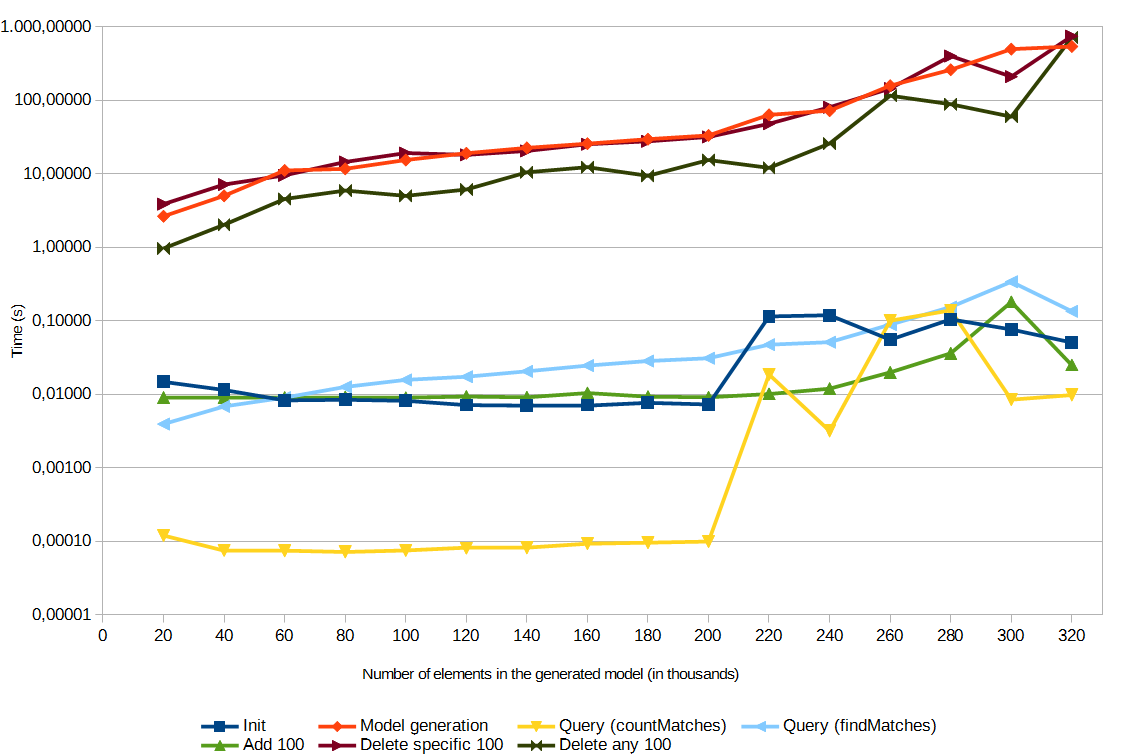
\includegraphics[width=\linewidth]{../common/figures/evaluation-runtime1-logarithmic}
	\caption{Runtime for Creation and Queries depending on Model Size}
	\label{fig:evaluation-runtime1}
\end{figure}

\noindent
After creating the models as described above, the model is queried for all standalone (simple) platforms and empty exits with the patterns \texttt{findStandalonePlatform} and \texttt{findEmptyExit} known from Section~\ref{application-conditions}.
Queries for the number of matches require a constant time, while queries for all matches have a linear overhead due to the conversion to typed matches.
Even for 320,000 matches the time is only 0.15~seconds.

As last insights, the time for adding 100 more platforms to the model of the given size and deleting them afterwards is shown.
The time for adding the platforms is independent of the current model size.
The deletion of the same 100 platforms is much more expensive, because this requires finding the matches for the pattern and filtering them for the ones with the respective platform (which will be exactly one in this case).
As there are many platforms, it takes a while to find the match which bounds the platform to be deleted -- the time for this step increases with the number of available matches, which is proportional to the model size in our example.
Deleting any 100 platforms instead of 100 specific ones takes less time, as matches for the patterns must not be filtered for the ones with the correct node binding.
The adding of elements also requires finding a match (in the pattern for creating a platform the game must be matched such that the containment edge between the game and the platform can be created), but as there is only one match this operation is faster than the deletion for which a lot of matches can be found.

For model sizes larger than 260,000 elements the measured runtimes vary a lot and the runtimes for model generation and deletion are not linear anymore.

For the performance tests presented in Figure~\ref{fig:evaluation-runtime1}, the API has been initialized with a resource set containing just one empty resource.
In this scenario, Democles cannot find any matches during the initialization (because the model contains no elements).
Whenever the model is changed by creating new elements, new matches are found and added to the maintained set of matches.

Figure~\ref{fig:evaluation-runtime2} illustrates the initialization of an API for loading existing models of different sizes (instead of starting with an empty model).
In this case, Democles has to search for all matches of all patterns during the initialization -- the larger the model, the more matches will be found.
The time for updating the set of matches grows linear with the model size, while the time for the initialization seems to be worse than linear.
After the initialization and the first update, the queries can be answered in constant time (plus a small overhead for the conversion to typed matches when all matches are returned) just as before.

\begin{figure}[h!]
	\centering
	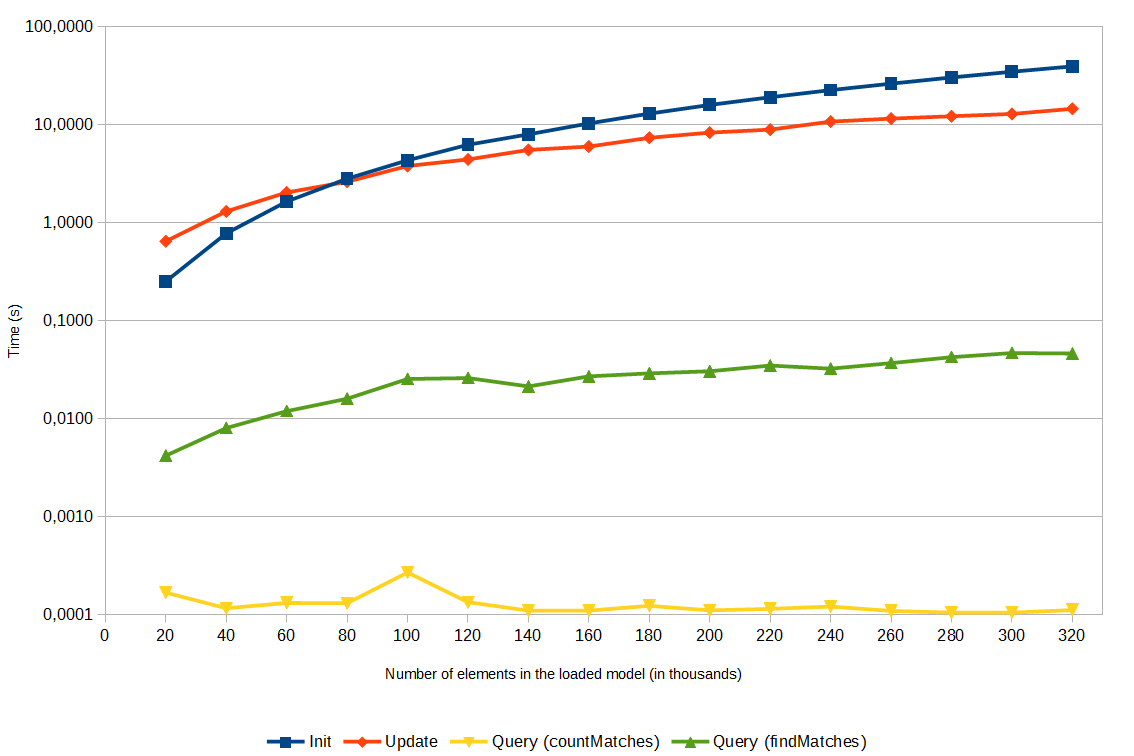
\includegraphics[width=\linewidth]{../common/figures/evaluation-runtime2-logarithmic}
	\caption{Runtime for Initialization and Queries depending on Model Size}
	\label{fig:evaluation-runtime2}
\end{figure}

\noindent
As the measurements only use one meta-model and the model has a certain structure (one root element with a lot of children), further tests are necessary to check whether the results can be generalized for arbitrary models.

In addition to the model size, the total number of observed patterns has a significant impact on the runtimes, as more patterns lead to larger times for searching the pattern structures and more matches to maintain.
The dependency on the size and complexity of the observed patterns (\eg number of nodes and edges in a pattern, usage of application conditions) has not been evaluated yet.

\section{Usability and End-User Feedback}
\label{evaluation-usability}
As eMoflon::IBeX-GT is intended to be used for teaching purposes, students using the tool in the lecture ``Model-Based Software Engineering'' (MBSE) and students writing their master's theses in the area of graph transformation were asked to give feedback via an online questionaire\footnote{\url{https://docs.google.com/forms/d/1r5pgkTv0CcvTQoqHlUuHcQqULl6A8CmbHgpt961BtHU}} being a mix of multiple choice and open questions.

\subsection{Experience of the participants}
20 students with a different level of experience with graph transformation, all members of our intended target group, participated in the survey (cp. Figure~\ref{fig:evaluation-results-experience-of-participants}).
Most of the participants have no or only little experience with graph transformation and model-driven engineering in general.
With one exception, all participants have programming experience and used the Eclipse IDE before.
Most participants are not familiar with visual (programming) languages.

\begin{figure}[h!]
	\centering
	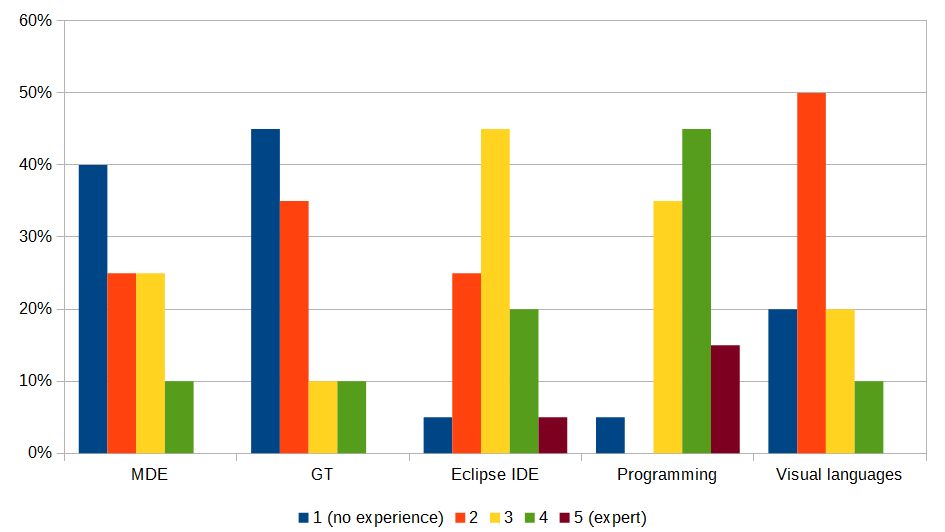
\includegraphics[width=\linewidth]{../common/figures/evaluation-results-experience-of-participants}
	\caption{Experience of the Participants}
	\label{fig:evaluation-results-experience-of-participants}
\end{figure}

\subsection{Textual and Visual Syntax}
\label{evaluation-syntax}
Figure~\ref{fig:evaluation-results-syntax} shows how the end-users rated the textual and visual syntax.
Most users think that the textual syntax is understandable (average 3.6 out of 5 stars, 90\,\% gave 3 or 4 stars).
Comments on the syntax are mostly positive, and highlight the visualization and the intuitive syntax.
For example, participants stated that the textual syntax ``easy to understand and write down'' and that ``the ++ and $--$ is intuitive, and there are no unnecessary chars like \texttt{;}''.

The participants especially like the mix of the textual and the visual syntax (average 4 stars, 70\,\% gave 4 or 5 stars).
The visualization (average 4.0 stars) is considered to be more helpful than the error messages (average 3.65 stars).
The usability of the editor as a whole is rated with 3.45 out of 5 stars on average, 90\,\% giving 3 or more stars.

Suggestions for improvements of the editor mainly focus on the visualization.
30\,\% would like to edit the visual syntax directly, which has not been implemented due to the complexity of visual editors (cp. the requirements).
They also point out that the overlapping of elements is an issue for large patterns.
As the layout of the visualization is handled by PlantUML, there seems to be only little potential for improvements with the current choice of visualization tool.

\begin{figure}[h!]
	\centering
	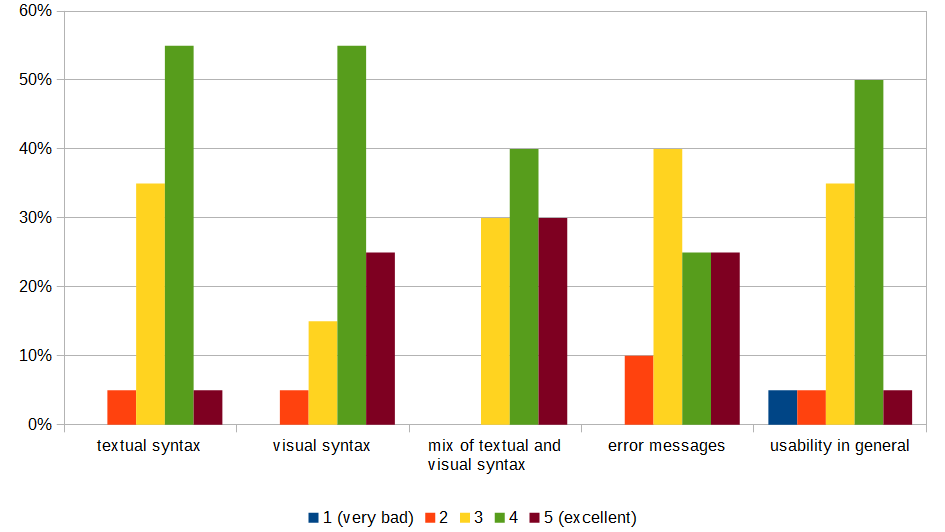
\includegraphics[width=\linewidth]{../common/figures/evaluation-results-syntax}
	\caption{Evaluation of Textual and Visual Syntax}
	\label{fig:evaluation-results-syntax}
\end{figure}

\subsection{Language Features}
\label{evaluation-features}
The users' estimation regarding the importance of selected language features is shown in Figure~\ref{fig:evaluation-results-importance-of-features}.
Complex graph conditions are the feature with the highest average rating (3.7), followed by application conditions (3.65) and attributes (3.55).
Pattern refinement and incrementality\footnote{The incremental features are called ``support for reactive programming'' in the survey because the participants of the survey do not know the details of the implementation based on incremental pattern matching.} are considered to be less important (2.9), which is surprising for us.

In our requirements list (Chapter~\ref{requirements}) we have considered incrementality and pattern refinement as the most important features, especially as there are no other graph transformation tools with support for those features.
One reason for this surprising result might be that the students asked for feedback only have a little experience with the tool and have not used all features in their own specifications yet.
Another important point is that both features make an impact for large applications maintained and evolved over a long time.

\begin{figure}[h!]
	\centering
	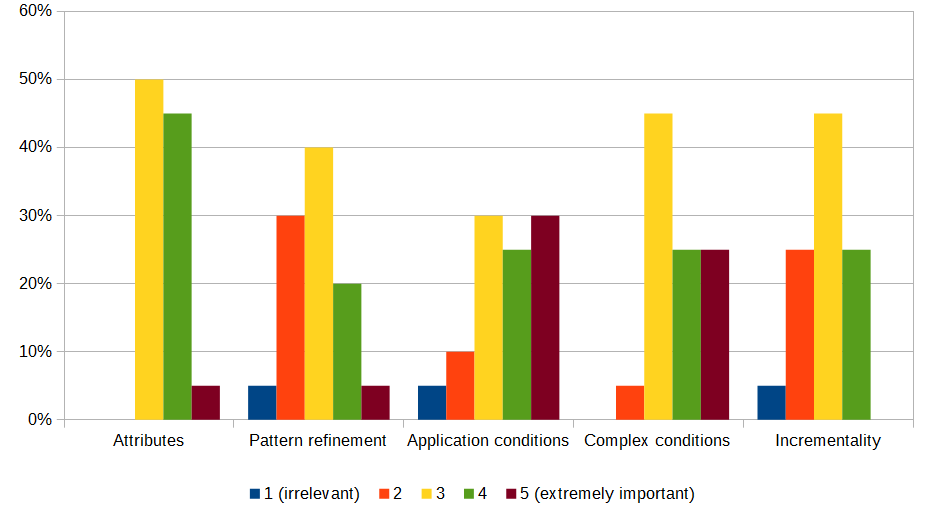
\includegraphics[width=\linewidth]{../common/figures/evaluation-results-importance-of-features}
	\caption{Importance of Language Features}
	\label{fig:evaluation-results-importance-of-features}
\end{figure}

\subsection{Potential for the Usage in Java Applications}
\label{evaluation-java-integration}
The users have been asked to comment on the integration with Java code.
Suggestions for improvements focus on a possibility to jump from the generated Java classes to the specification via one click (``Make it possible to directly navigate to the patterns/rules from the code''), although switching between \texttt{gt} files and the Java classes is a quite seamless experience from the point view of 35\,\% of the participants, and average for another 55\,\% of them.
As this gets more complex when the specification consists of many \texttt{gt} files, a linking between editor patterns/rules and Java classes is planned for the future.

Most users think that the pattern language is expressive enough to specify patterns of realistic complexity in practice (average 3.55 out of 5 stars).
Almost a two-third majority voted with 4 or 5 stars.

Asked for the main arguments for using eMoflon::IBeX-GT in a Java project many students named the visualization, as this makes the specification understandable for non-programmers.
Furthermore, one user commented: ``Using patterns is closer to the underlying model, easier to adapt to changes, less error-prone and much less work than hard-coding the operations on the EMF model''.
Drawbacks in the users' opinion are performance, a more complex project setup (considered to be costly especially for small projects) and a missing debugging facility.
Actually, debugging is possible via analyzing the pattern specifications and the received matches.

\begin{figure}[h!]
	\centering
	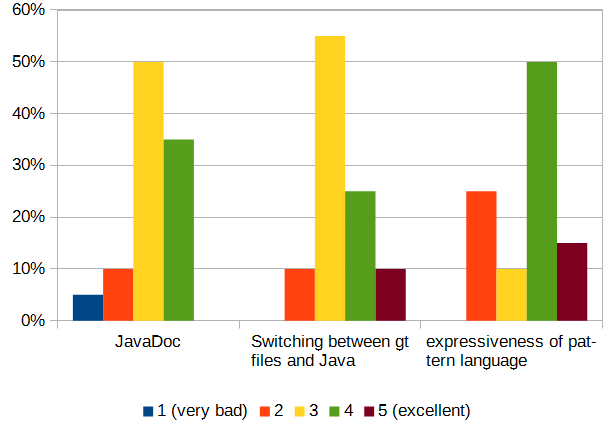
\includegraphics[width=0.65\linewidth]{../common/figures/evaluation-results-java-integration}
	\caption{Evaluation of the Potential for the Usage in Java Applications}
	\label{fig:evaluation-results-java-integration}
\end{figure}

\subsection{Handbook}
\label{evaluation-handbook}
The handbook \cite{eMoflonIBeX-GT-Handbook} introduces eMoflon::IBeX-GT by developing an example application (``Sokoban'') step by step.
In an appendix all features of the pattern language and the API are explained, as not all of them are used in the example.
The students enjoyed working through the handbook (``fun factor'' average 4.0 out of 5 stars).
The appendix is rated as average by most students.
The students were asked for feedback after working through the tutorial, which does not require the appendix.
The pattern and API references in the appendix are considered for advanced users who need to lookup some details.

\begin{figure}[h!]
	\centering
	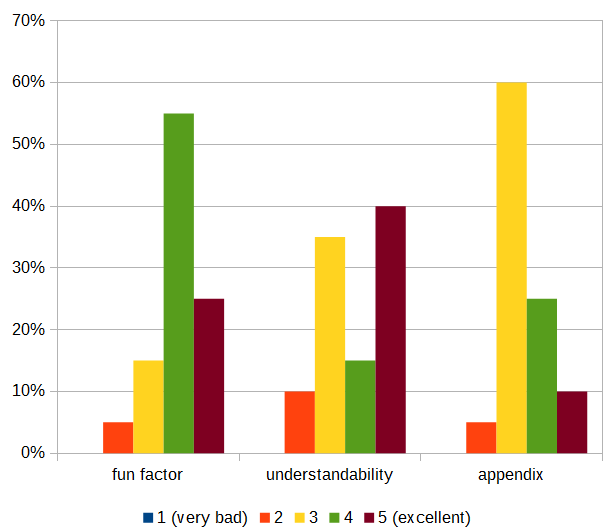
\includegraphics[width=0.65\linewidth]{../common/figures/evaluation-results-handbook}
	\caption{Evaluation of the Handbook}
	\label{fig:evaluation-results-handbook}
\end{figure}
